\documentclass[11pt]{article}
\usepackage[margin=0.7in]{geometry}
\usepackage{multirow}
\usepackage {graphicx}
\usepackage[utf8x]{inputenc} % указать кодировку русского текста
\usepackage[russian]{babel} % указать, что язык текста - русский
\usepackage{fancyhdr}
\pagestyle{fancy}

\begin{document}

\begin{titlepage}

\begin{center}
%\vspace*{1cm}
\large\textbf{Московский Физико-Технический Институт}\\
\large\textbf{(государственный университет)}
\vfill
\line(1,0){430}\\[1mm]
\huge\textbf{Исследование взаимной диффузии газов}\\
\line(1,0){430}\\[1mm]
\vfill
\large Сибгатуллин Булат, ФРКТ\\
\end{center}

\end{titlepage}

\fancyhead[L] {Работа 2.2.1}
\noindent \textbf{Цель работы:} \\
\indent 1)  регистрация  зависимости  концентрации   гелия в воздухе от времени с помощью датчиков теплопроводности при разных начальных давлениях смеси газов; 2) определение коэффициента диффузии по результатам измерений.\\
\noindent \textbf{В работе используются:} \\
\indent измерительная установка; форвакуумный насос; баллон с газом (гелий); манометр; источник питания; магазин сопротивлений; гальванометр; секундомер.

\section*{Описание работы}\

Диффузия в системе, подчиняется закону Фика. В одномерном случае его можно записать так:

\[j_a = -D \frac{\partial n_a}{\partial x}, \quad j_b = -D \frac{\partial n_b}{\partial x},\]

где D - коэффициент взаимной диффузии  компонентов. Знак «минус» отражает тот факт, что диффузия идёт в направлении выравнивания концентраций.

В данной работе исследуется взаимная диффузия гелия и воздуха. Давление P и температура T в условиях опыта предполагаются неизменными.  Для любых изменений концентраций справедливо $\bigtriangleup n_b = -\bigtriangleup n_{he}$. Следовательно, достаточно ограничиться описанием диффузии одного из компонентов, например гелия:

\begin{equation}
j_{he} = -D \frac{\partial n_{he}}{\partial x}
\end{equation}

Перемешивание газов в работе можно приближенно описывать как диффузию примеси лёгких частиц He на практически стационарном фоне воздуха. Коэффициент диффузии в таком приближении равен:

\begin{equation}
D = \frac{1}{3} \lambda \overline{v},
\end{equation}

где $\overline{v} = \sqrt{\frac{8RT}{\pi \mu}}$ - средняя тепловая скорость частиц примеси, $\lambda = \frac{1}{n_0 \sigma}$ - их длина свободного пробега, $n_0$ - концентрация рассеивающих центров, $\sigma$ - сечение столкновения частиц примеси с частицами фона.

\vspace{0.5cm}

Применяя закон Фика для нашей установки можем найти распределении концентрации в трубке $n(x)$ - линейная функция:

\[j = - D \frac{\partial n}{\partial x} = const.\]

\begin{equation}
n(x) = \frac{\bigtriangleup n}{L} x
\end{equation}

и плотность потока частиц всюду постоянна и равна

\begin{equation}
j = -D \frac{\bigtriangleup n}{L}
\end{equation}

$\bigtriangleup n$ - разность концентраций гелия на концах трубки.

Можем посчитать количеств частиц, пересекающих в единицу времени любое поперечное сечение трубки, зная площадь сечения трубки S:

\begin{equation}
\frac{dN_1}{dt} = jS, \quad \frac{dN_2}{dt} - jS
\end{equation}

Выразим отсюда скорость изменения $\bigtriangleup n$. Вычитая из второго равенства
первое и деля результат на объём сосуда V , с учетом (4) получим

\begin{equation}
\frac{d (\bigtriangleup n)}{dt} = - \frac{\bigtriangleup n}{\tau}
\end{equation}

где введено обозначение

\begin{equation}
\tau = \frac{1}{D} \frac{VL}{2 S}
\end{equation}

Интегрируя (6), получаем, что разность концентраций будет убывать по экспоненциальному закону

\begin{equation}
\bigtriangleup n = \bigtriangleup n_0 e^{-t/\tau}
\end{equation}

где $\bigtriangleup n_0$ - разность концентраций примеси в сосудах в начальный момент
времени.

На установке мы измеряем напряжение, оно пропорционально разности концентраций, следовательно:

\begin{equation}
U = U_0 e^{-t/\tau}
\end{equation}

\section*{Оборудование}\
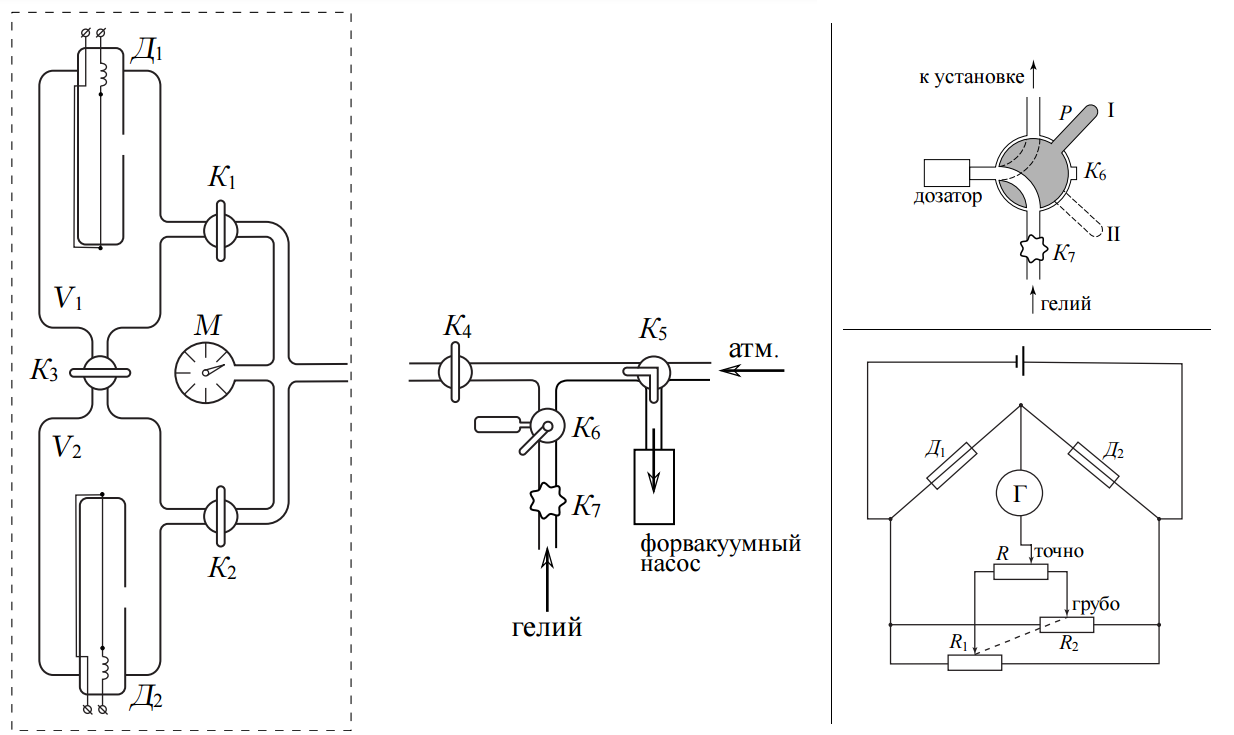
\includegraphics[scale=0.4]{pic1.png}

\newpage

\section*{Ход работы}\

\vspace{0.5cm}

Запишем параметры установки:

\[V = 800 \pm 5 \: \textit{см}^3\]

\[L/S = 15,0 \pm 0,1 \: \textit{см}^{-1}\]

\[P_{he} = 0,2 P, \quad P_{vos} = 1,75 P\]

Проведем измерения и запишем данные в таблицу:

\vspace{0.5cm}

\begin{figure}[h!]
\centering
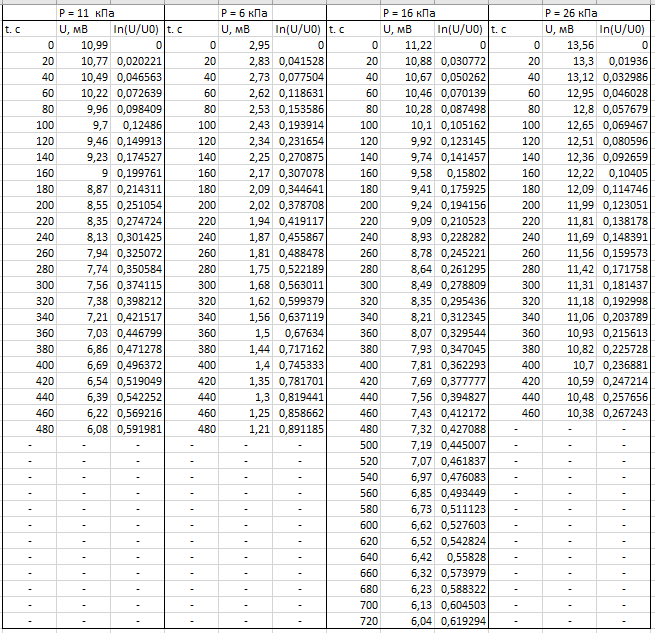
\includegraphics[scale=1.4]{table.png}
\label{fig:Image1}
\end{figure}

При помощи МНК построим графики линейной зависимости в координатах $-ln (U/U_0)$, $t$:

\[ b = \frac{<xy> - <x><y>}{<x^2> - <x>^2}\]

\[a =<y> - b<x>\]

\[\sigma_b = \frac{1}{\sqrt{n}} \sqrt { \frac{<y^2> - <y>^2}{<x^2> - <x>^2}  - b^2}\]

\[\sigma_a = \sigma_b \sqrt{<x^2> - <x>^2}\]

\vspace{0.5cm}

Зная, что $b = 1/\tau$ будем сразу искать значение для коэффициента диффузии.

Для P = 6 кПа

\[b_1 = 0,00185 \pm 0,00005 \: \textit{с}^{-1}\]

\[D_1 = \frac{1}{\tau} \frac{VL}{2S} = b_1 \frac{VL}{2S} = 0,00185 \cdot \frac{800}{2} \cdot 15 = 11,10\]

\[\sigma_{D_1} = D_1 \sqrt{\Big( \frac{\sigma_{b_1}}{b_1} \Big)^2 + \Big( \frac{\sigma_V}{V} \Big)^2 + \Big( \frac{\sigma_{L/S}}{L/S} \Big)^2} = 11,1 \cdot \sqrt{\Big( \frac{0,00005}{0,00185} \Big)^2 + \Big( \frac{5}{800} \Big)^2 + \Big( \frac{0,1}{15} \Big)^2} = 0,32\]

\[D_1 = 11,10 \pm 0,32\]

\vspace{0.5cm}

Для P = 11 кПа

\[b_2 = 0,00124 \pm 0,00004 \: \textit{с}^{-1}\]

\[D_2 = \frac{1}{\tau} \frac{VL}{2S} = b_2 \frac{VL}{2S} = 0,00124 \cdot \frac{800}{2} \cdot 15 = 7,44\]

\[\sigma_{D_2} = D_2 \sqrt{\Big( \frac{\sigma_{b_2}}{b_2} \Big)^2 + \Big( \frac{\sigma_V}{V} \Big)^2 + \Big( \frac{\sigma_{L/S}}{L/S} \Big)^2} = 7,44 \cdot \sqrt{\Big( \frac{0,00004}{0,00124} \Big)^2 + \Big( \frac{5}{800} \Big)^2 + \Big( \frac{0,1}{15} \Big)^2} = 0,25\]

\[D_2 = 7,44 \pm 0,25\]

\vspace{0.5cm}

Для P = 16 кПа

\[b_3 = 0,000843 \pm 0,000041 \: \textit{с}^{-1}\]

\[D_3 = \frac{1}{\tau} \frac{VL}{2S} = b_3 \frac{VL}{2S} = 0,000843 \cdot \frac{800}{2} \cdot 15 = 5,06\]

\[\sigma_{D_3} = D_3 \sqrt{\Big( \frac{\sigma_{b_3}}{b_3} \Big)^2 + \Big( \frac{\sigma_V}{V} \Big)^2 + \Big( \frac{\sigma_{L/S}}{L/S} \Big)^2} = 5,06 \cdot \sqrt{\Big( \frac{0,000041}{0,000843} \Big)^2 + \Big( \frac{5}{800} \Big)^2 + \Big( \frac{0,1}{15} \Big)^2} = 0,25\]

\[D_3 = 5,06 \pm 0,25\]

\vspace{0.5cm}

Для P = 26 кПа

\[b_4 = 0,00567 \pm 0,000044 \: \textit{с}^{-1}\]

\[D_4 = \frac{1}{\tau} \frac{VL}{2S} = b_4 \frac{VL}{2S} = 0,000567 \cdot \frac{800}{2} \cdot 15 = 3,41\]

\[\sigma_{D_4} = D_4 \sqrt{\Big( \frac{\sigma_{b_4}}{b_4} \Big)^2 + \Big( \frac{\sigma_V}{V} \Big)^2 + \Big( \frac{\sigma_{L/S}}{L/S} \Big)^2} = 3,41 \cdot \sqrt{\Big( \frac{0,000044}{0,000567} \Big)^2 + \Big( \frac{5}{800} \Big)^2 + \Big( \frac{0,1}{15} \Big)^2} = 0,26\]

\[D_4 = 3,41 \pm 0,26\]

\vspace{0.5cm}

По полученным значениям построим график в координатах $D(1/P)$ при помощи МНК. Для построения графика определим погрешность $1/P$, зная, что погрешность $\sigma_P = 0,5$ кПа:

\[\frac{1}{P_1} = \frac{1}{6000} = 1,67 \cdot 10^{-4} \: \textit{Па}^{-1}\]

\[\sigma_{1/P_1} = \frac{1}{P_1} \cdot \sqrt{\Big( \frac{\sigma_P}{P_1} \Big)^2} = \frac{1}{6000} \cdot \sqrt{\Big( \frac{0,5}{6} \Big)^2} = 1,4 \cdot 10^{-5} \:  \textit{Па}^{-1}\]

\[\frac{1}{P_1} = (1,67 \pm 0,14) \cdot  10^{-4} \: \textit{Па}^{-1}\]

\begin{figure}[h!]
\centering
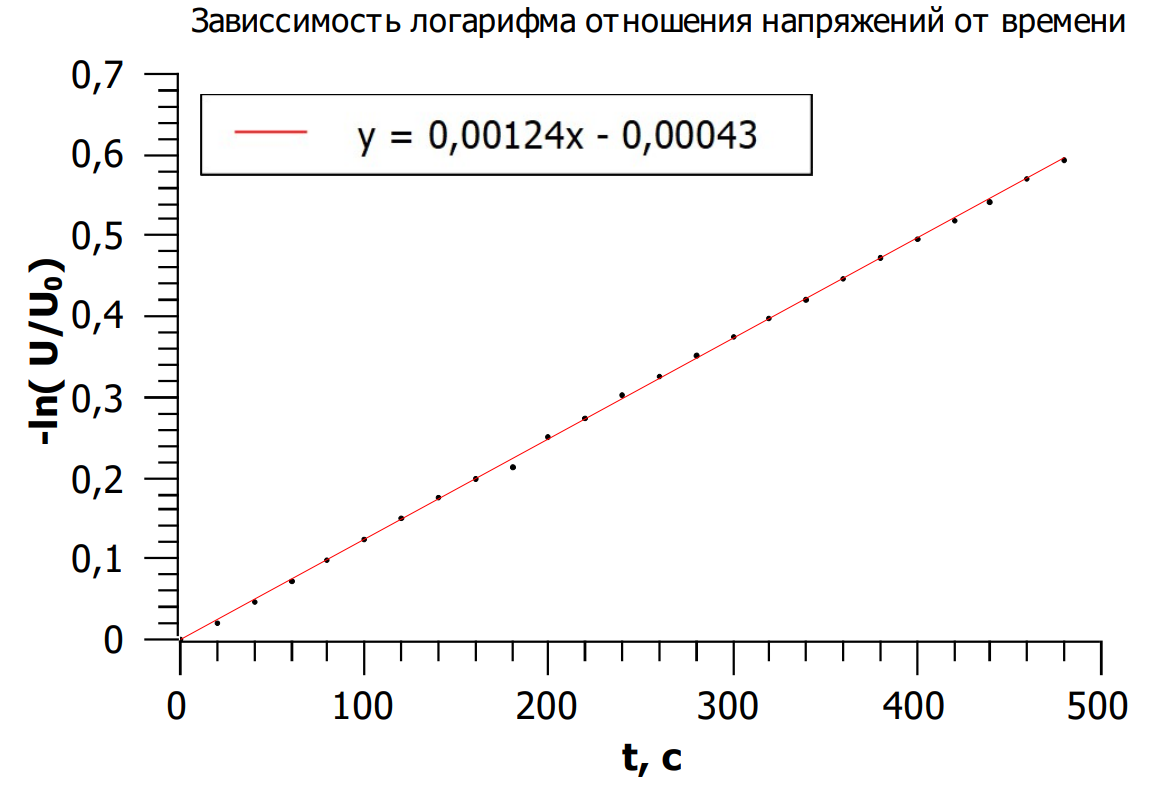
\includegraphics[scale=0.6]{1graph.png}
\label{fig:Image1}
\end{figure}

\begin{figure}[h!]
\centering
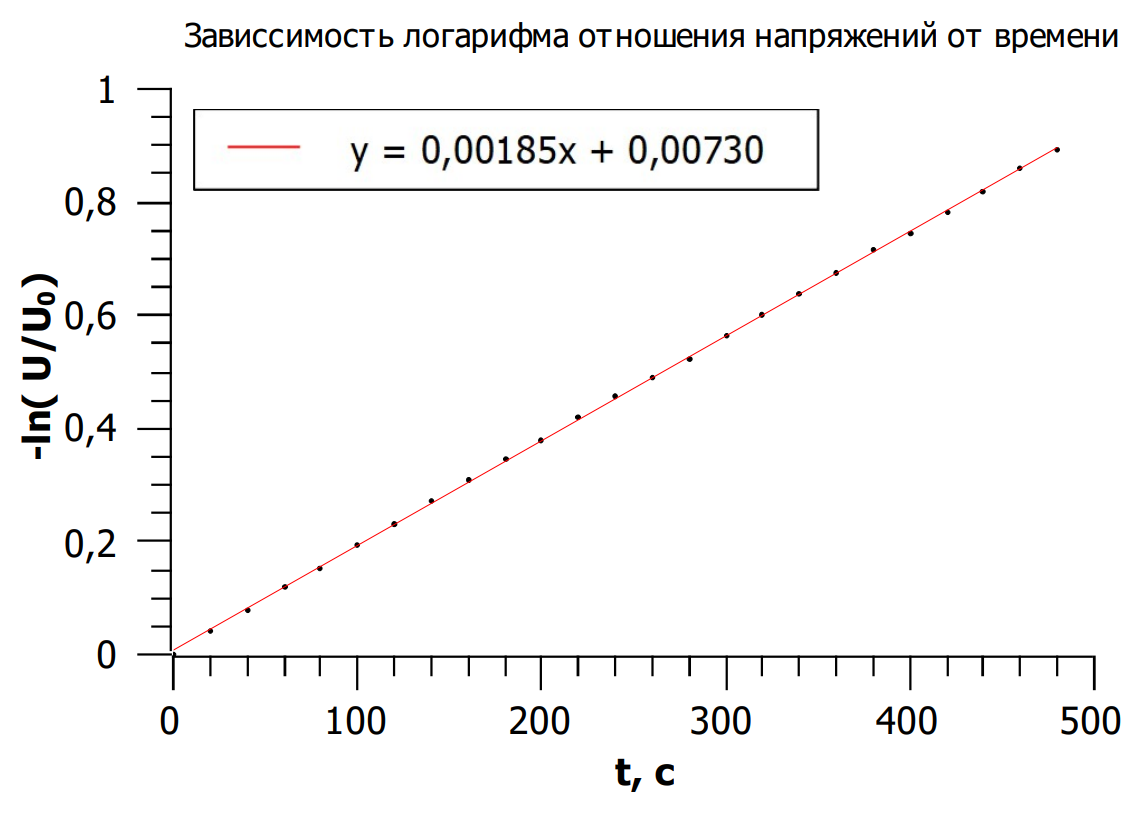
\includegraphics[scale=0.6]{2graph.png}
\label{fig:Image1}
\end{figure}

\begin{figure}[h!]
\centering
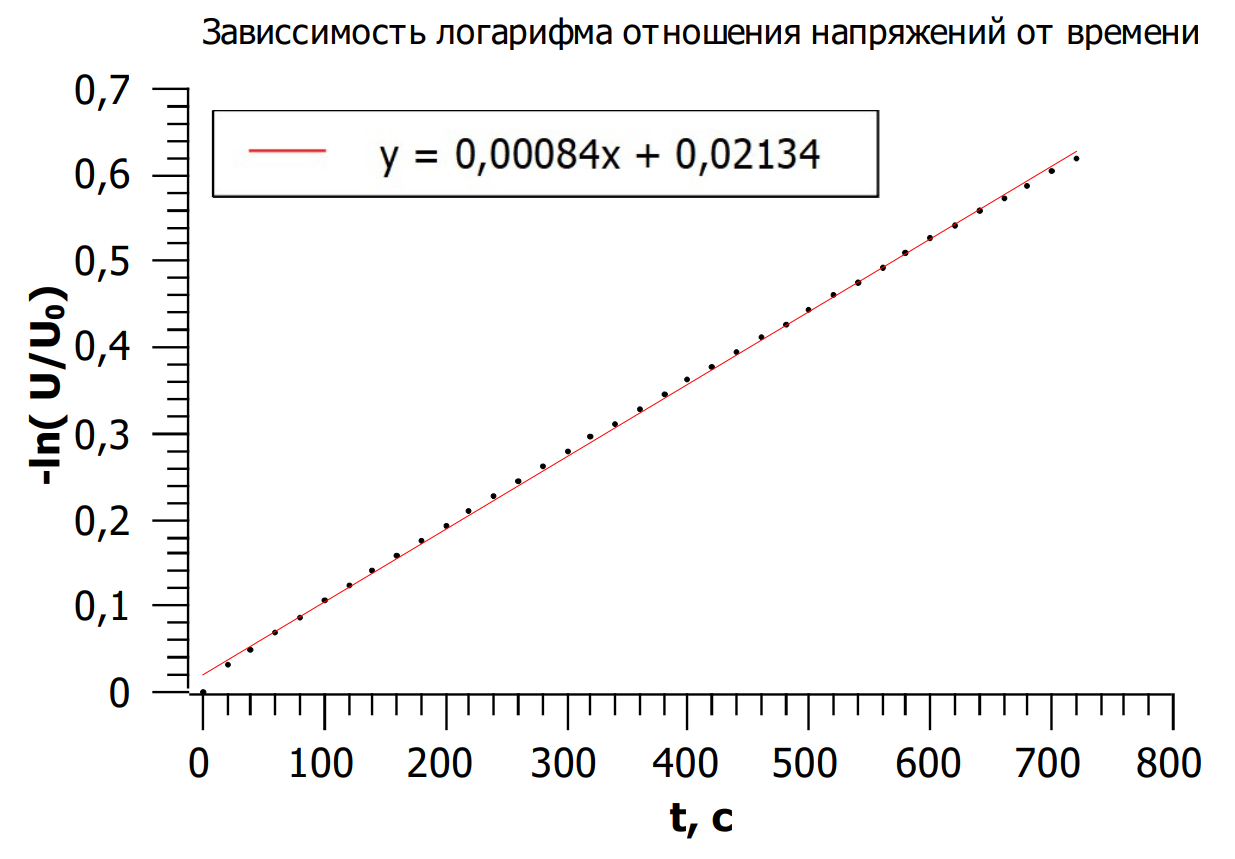
\includegraphics[scale=0.6]{3graph.png}
\label{fig:Image1}
\end{figure}

\begin{figure}[h!]
\centering
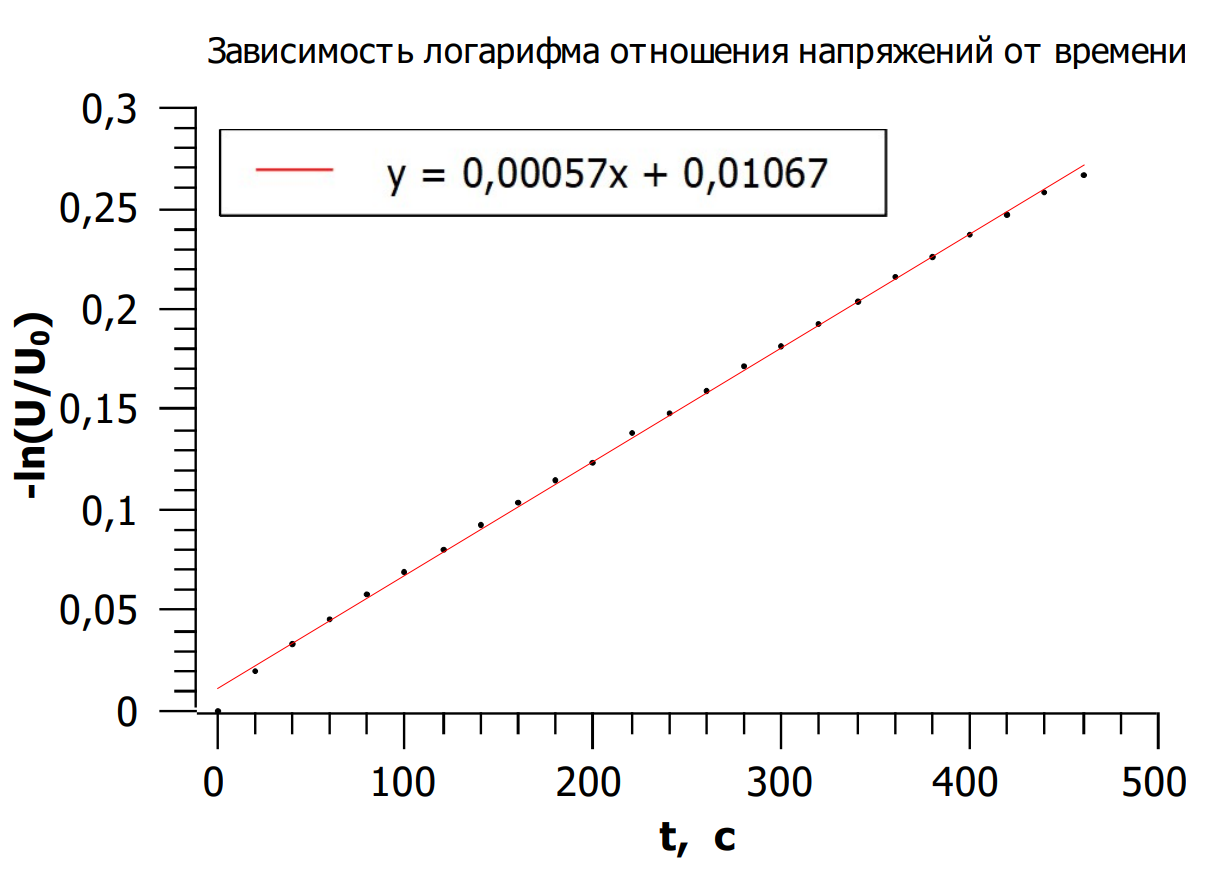
\includegraphics[scale=0.6]{4graph.png}
\label{fig:Image1}
\end{figure}

\vspace{0.3cm}

\[\frac{1}{P_2} = \frac{1}{11000} = 9,1 \cdot 10^{-5} \: \textit{Па}^{-1}\]

\[\sigma_{1/P_2} = \frac{1}{P_2} \cdot \sqrt{\Big( \frac{\sigma_P}{P_2} \Big)^2} = \frac{1}{11000} \cdot \sqrt{\Big( \frac{0,5}{11} \Big)^2} = 4,1 \cdot 10^{-6} \: \textit{Па}^{-1}\]

\[\frac{1}{P_2} = (9,1 \pm 0,41) \cdot  10^{-5} \: \textit{Па}^{-1}\]

\vspace{0.3cm}

\[\frac{1}{P_3} = \frac{1}{16000} = 6,25 \cdot 10^{-5} \: \textit{Па}^{-1}\]

\[\sigma_{1/P_3} = \frac{1}{P_3} \cdot \sqrt{\Big( \frac{\sigma_P}{P_3} \Big)^2} = \frac{1}{16000} \cdot \sqrt{\Big( \frac{0,5}{16} \Big)^2} = 1,9 \cdot 10^{-6} \: \textit{Па}^{-1}\]

\[\frac{1}{P_3} = (6,25 \pm 0,19)\cdot  10^{-5} \:\textit{Па}^{-1}\]

\vspace{0.3cm}

\[\frac{1}{P_4} = \frac{1}{26000} = 3,84 \cdot 10^{-5} \: \textit{Па}^{-1}\]

\[\sigma_{1/P_4} = \frac{1}{P_4} \cdot \sqrt{\Big( \frac{\sigma_P}{P_4} \Big)^2} = \frac{1}{26000} \cdot \sqrt{\Big( \frac{0,5}{26} \Big)^2} = 7,4 \cdot 10^{-7} \: \textit{Па}^{-1}\]

\[\frac{1}{P_4} = (3,84 \pm 0,07) \cdot  10^{-5} \: \textit{Па}^{-1}\]

\begin{figure}[h!]
\centering
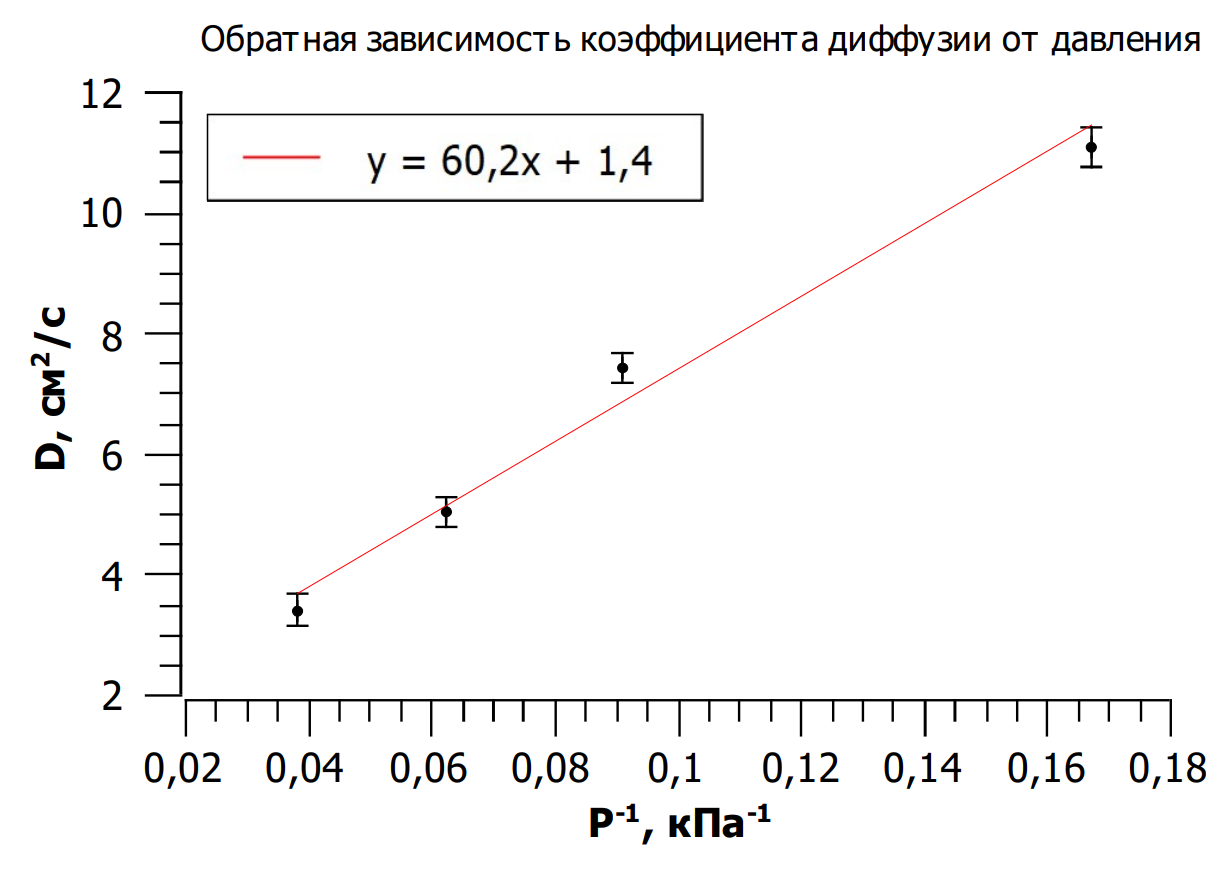
\includegraphics[scale=0.6]{D.png}
\label{fig:Image1}
\end{figure}

При помощи МНК построим график и запишем угловой коэффициент:

\vspace{0.3cm}

\[b = \frac{<xy> - <x><y>}{<x^2> - <x>^2}\]

$b = \frac{(0,038 \cdot 3,41 + 0,625 \cdot 5,06 + 0,091 \cdot 7,44 + 0,167 \cdot 11,1) - (0,038 + 0,0625 + 0, 091 + 0,167) \cdot (3,41 + 5,06 + 7,44 + 11,1)}{(0,038^2 + 0,0625^2 + 0,091^2 + 0,167^2) - (0,038 + 0,0625 + 0, 091 + 0,167)^2}$

\[b = 60,2\]

\[a =<y> - b<x>\]

$a = (3,41 + 5,06 + 7,44 + 11,1) - 60,2 \cdot (0,038 + 0,0625 + 0, 091 + 0,167) $

\[a = 1,39\]

\[\sigma_b = \frac{1}{\sqrt{n}} \sqrt { \frac{<y^2> - <y>^2}{<x^2> - <x>^2}  - b^2}\]

$\sigma_b = \frac{1}{2} \sqrt{\frac{(3,41^2 + 5,06^2 + 7,44^2 + 11,1^2) - (3,41 + 5,06 + 7,44 + 11,1)^2}{(0,038^2 + 0,0625^2 + 0,091^2 + 0,167^2) - (0,038 + 0,0625 + 0, 091 + 0,167)^2}}$

\[\sigma_b = 3,1\]

\[\sigma_a = \sigma_b \sqrt{<x^2> - <x>^2}\]

$\sigma_a = 3,1 \sqrt{(0,038^2 + 0,0625^2 + 0,091^2 + 0,167^2) - (0,038 + 0,0625 + 0, 091 + 0,167)^2}$

\[\sigma_a = 0,28\]

Запишем в виде интервала:

\[b = 60,2 \pm 3,1\]

\[a = 1,39 \pm 0,28\]

Проэкстраполировав к $P = 10^5$ Па, получаем:

\[D = (0,602 \pm 0,031) \: \textit{см}^2/\textit{c}\]

Вычислим $\lambda$:

\[D=\frac{1}{3}\lambda <v>, \quad <v>=\sqrt{\frac{8RT}{\pi \mu}}\]

\[\lambda = 3D \sqrt{\frac{\pi \mu}{8RT}} = 3 \cdot 0,6 \cdot 10^{-4} \frac{3,14 \cdot 4 \cdot 10^{-3}}{8\cdot 8,31 \cdot 293} = 1,46 \cdot 10^{-7} \: \textit{м}\]

\[\sigma_{\lambda} = \lambda \sqrt{\Big( \frac{\sigma_D}{D} \Big)^2} = 1,77 \cdot 10^{-6} \cdot \sqrt{\Big( \frac{0,031}{0,602} \Big)^2} = 7,5 \cdot 10^{-9} \: \textit{м}\]

\[\lambda = (1,46 \pm 0,08) \cdot 10^{-7} \: \textit{м}\]


\section*{Вывод}\

Определили зависимость коэффициента дифузии от давления и посчитали коэффициент диффузии для атмосферного давления. Оценили длину свободного пробега атомов гелия в воздухе. 

\end{document}